\documentclass[a4paper,onesided,12pt]{report}
\usepackage{styles/fbe_tez}
\usepackage[utf8]{inputenc} % Unicode (e.g. Turkish); utf8x removed from TeX Live 2020+
\renewcommand{\labelenumi}{(\roman{enumi})}
\usepackage{amsmath, amsthm, amssymb}
 % Some extra symbols
\usepackage[bottom]{footmisc}
\usepackage{cite}
\usepackage{url}
\usepackage{graphicx}
\usepackage{longtable}
\graphicspath{{figures/}} % Graphics will be here

%\usepackage{xtab}
\usepackage{multirow}
\usepackage{subfigure}
\usepackage{float}
\usepackage{placeins}
%\pagestyle{empty}
%\includeonly{introduction} % To only process the given file

\newtheorem{thm}{Theorem}[chapter]
\newtheorem{prop}[thm]{Proposition}
\newtheorem{lem}[thm]{Lemma}
\newtheorem{cor}[thm]{Corollary}
% COVER PAGE
\title{Edge deployment: Plant health classification (MobileNet V3) on Raspberry Pi Zero 2 W}
\author{Yusuf Savaş \\ Advisor: Fikret Gürgen}



\begin{document}

\pagenumbering{roman}
\maketitle{}
\tableofcontents

\pagenumbering{arabic}

\chapter{Introduction}

Plant pests and diseases destroy up to \textbf{40\%} of global crop production each year and cost the world economy about \textbf{US\$220 billion} annually~\cite{fao2021pests}; major staple crops see \textbf{10--40\%} yield losses to pathogens~\cite{savary2019global}. Catching disease early from a leaf image enables timely treatment, less blanket pesticide use, and better yield protection, especially for smallholders who rarely have fast access to a pathologist.

We build an \textbf{edge-deployed} classifier on a \textbf{Raspberry Pi Zero 2 W}~\cite{raspberrypi_zero2w}: a camera image is labeled \textbf{healthy}, \textbf{diseased}, or \textbf{background} (non-leaf) using \textbf{MobileNet V3}~\cite{howard2019mobilenetv3} exported to \textbf{ONNX}~\cite{onnx} and run with \textbf{ONNX Runtime}~\cite{onnxruntime} from \textbf{C++} for predictable, low-memory inference. The main focus points are:
\begin{itemize}
\item Train on public leaf and background data, then deploy the same preprocessing and graph on the Pi.
\item Measure \textbf{accuracy and throughput} on device (FP32 baseline vs.\ \textbf{INT8} quantization~\cite{jacob2018quantization}).
\item Expose results through a \textbf{web portal} and validate with a \textbf{real camera}, test bench, and field-style captures,not only dataset images.
\end{itemize}

\chapter{Description}

\section{Hardware}

\textbf{Raspberry Pi Zero 2 W} was chosen as a \textbf{low-cost, resource-constrained} edge node:

\begin{table}[htbp]
\centering
\begin{tabular}{|l|p{0.62\textwidth}|}
\hline
\textbf{Item} & \textbf{Detail} \\
\hline
CPU & Quad-core ARM Cortex-A53 ($\sim$1\,GHz) \\
\hline
RAM & 512\,MB \\
\hline
Inference & CPU only (no GPU or NPU) \\
\hline
\end{tabular}
\end{table}

\section{Software}

\begin{itemize}
\item \textbf{Model}: \textbf{MobileNet V3}~\cite{howard2019mobilenetv3} exported to \textbf{ONNX}~\cite{onnx} for deployment.
\item \textbf{Runtime}: \textbf{ONNX Runtime}~\cite{onnxruntime} used from \textbf{C++}
\item \textbf{Pipeline}: \textbf{Image in $\rightarrow$ MobileNet-style preprocessing $\rightarrow$ ONNX Runtime inference $\rightarrow$ class scores / label}.
\item \textbf{Web UI}: a \textbf{web portal} on the device (or on the LAN) shows \textbf{camera view}, \textbf{live predictions}, \textbf{summary metrics}, and \textbf{throughput (FPS or images per second)}.
\end{itemize}

\section{Use}

In practice the app does one thing: from a picture of a leaf it guesses whether the plant looks \textbf{healthy} or \textbf{unhealthy}.

For a \textbf{demo}, you open the \textbf{web page} on your phone or laptop (on the same Wi-Fi as the device). You show \textbf{healthy} and \textbf{unhealthy} plants to the camera, or step through example images, and everyone can see the \textbf{label} the model picked and \textbf{how many frames per second} it is running.

\section{Diagram}

\IfFileExists{figures/system_architecture.pdf}{%
  Figure~\ref{fig:system-architecture} shows the logical data flow.
  \begin{figure}[h!]
  \centering
  
\includegraphics[width=0.95\textwidth]{system_architecture.pdf}
  \caption{System architecture: camera and files into preprocess, ONNX Runtime, web portal, and browser on the LAN.}
  \label{fig:system-architecture}
  \end{figure}
}{%
  \begin{quote}
  \textit{Build the figure first: from \path{results/report/}, run \path{./render-mermaid.sh} (needs Node and \path{@mermaid-js/mermaid-cli}, or a global \path{mmdc}).}
  \end{quote}
}

\chapter{Requirements}

\section{Features}

\begin{itemize}
\item Open a \textbf{web portal} and see \textbf{inference results} (predicted class and, where applicable, confidence).
\item See \textbf{performance at a glance}: \textbf{FPS} (or equivalent throughput) and, if useful, \textbf{per-frame or rolling latency}, updated as the system runs.
\item Run \textbf{single-image} or \textbf{stream/batch} inference through the same stack so lab tests and field-style runs share one pipeline.
\end{itemize}

\textbf{Layers}

\begin{table}[h!]
\begin{center}
\begin{tabular}{|l|p{9cm}|}
\hline
\textbf{Layer} & \textbf{Role} \\
\hline
\textbf{Presentation} & Web UI (portal) for status, predictions, FPS, and optional history or session summary. \\
\hline
\textbf{Application / API} & Serves the UI and exposes inference status and metrics to it (WebSocket). \\
\hline
\textbf{Inference} & Loads the \textbf{MobileNet V3 ONNX} graph, applies consistent preprocessing, runs \textbf{ONNX Runtime} on the device CPU. \\
\hline
\textbf{Acquisition (optional path)} & Feeds frames from storage or from a \textbf{camera} into the preprocessor; same graph for file replay and live capture when implemented. \\
\hline
\textbf{Quantization track} & Same topology with \textbf{INT8} weights for comparison against the \textbf{FP32} baseline, with accuracy and speed measured under identical UI and metrics. \\
\hline
\end{tabular}
\end{center}
\end{table}

\textbf{Offline tests}

\begin{itemize}
\item Ability to score a \textbf{fixed labeled test split} and report \textbf{classification metrics} (accuracy, balanced accuracy, precision/recall/F1 for the diseased class, specificity) and a \textbf{confusion matrix}, independent of the portal, for rigorous comparison between FP32 and INT8 builds.
\end{itemize}

\chapter{Designed System}

\section{Choices}

\begin{itemize}
\item \textbf{MobileNet V3}~\cite{howard2019mobilenetv3} balances accuracy and a small parameter count (\textbf{1{,}519{,}906} parameters in the trained checkpoint) for edge use.
\item \textbf{ONNX + ONNX Runtime}~\cite{onnx,onnxruntime} provides a \textbf{deployment-oriented} graph and a runtime tuned for multiple backends; a \textbf{native} caller keeps measurements close to how the stack would ship in production.
\item \textbf{FP32 baseline first}, then \textbf{INT8} (or similar) as a controlled experiment: smaller artifacts and faster integer math on CPU, with accuracy tracked against the same test protocol.
\item \textbf{Web portal} as the default way to \textbf{see results and FPS} aligns the system with operator expectations and simplifies demos and field checks.
\end{itemize}

\section{Pipeline}

\begin{enumerate}
\item \textbf{Input}: image from file, batch folder, or (when available) camera frame.
\item \textbf{Preprocess}: resize and normalize to match training/export conventions.
\item \textbf{Inference}: ONNX Runtime executes the graph on the CPU.
\item \textbf{Output}: class prediction (and optional scores); metrics feed the \textbf{portal} and any batch evaluator.
\item \textbf{Presentation}: portal displays \textbf{prediction}, \textbf{FPS / throughput}, and optional aggregates.
\end{enumerate}

\section{Quantization}

A reduced-precision build (e.g.\ \textbf{INT8} weight quantization) targets \textbf{smaller footprint and faster inference} on the same CPU, with \textbf{accuracy and FPS} compared to the \textbf{FP32} baseline under the same preprocessing and portal-facing metrics.

\chapter{Implementation}

The system is built in two stages that share the same image representation, so results obtained on the workstation carry over to the device. First, a model is trained and exported on a development workstation. Second, an on-device runtime loads that model and serves a web portal on the Raspberry Pi. Both stages feed the network the same input: a $224\times224$ RGB image, normalized with the standard ImageNet statistics, so the on-device numbers are directly comparable to the reference evaluation.

\section{Data preparation}

The classifier is trained on a three-class dataset: \textbf{healthy}, \textbf{diseased}, and \textbf{background}. The leaf classes come from \textbf{PlantVillage}~\cite{hughes2015plantvillage}, a large public collection of single-leaf photographs taken on a plain background. PlantVillage originally labels leaves with 38 fine-grained categories (crop $\times$ disease); for this work those are collapsed into a binary health signal: any leaf marked as healthy becomes \textbf{healthy}, and every other label becomes \textbf{diseased}.

A model trained only on clean leaf photos has no way to say ``this is not a leaf,'' which is a problem for a live camera that constantly sees hands, tables, and clutter. To handle this, a \textbf{background} class is added from \textbf{COCO 2017}~\cite{lin2014coco}, a dataset of everyday non-leaf scenes, supplemented with a small fraction of synthetic background images. This lets the deployed model reject non-leaf input instead of being forced to guess healthy or diseased.

The combined dataset is split \textbf{70\,/\,15\,/\,15} into training, validation, and test sets, keeping the three classes separated so that accuracy can be measured on images the model never saw during training.

\begin{figure}[H]
\centering
\subfigure[PlantVillage leaf samples (healthy / diseased)]{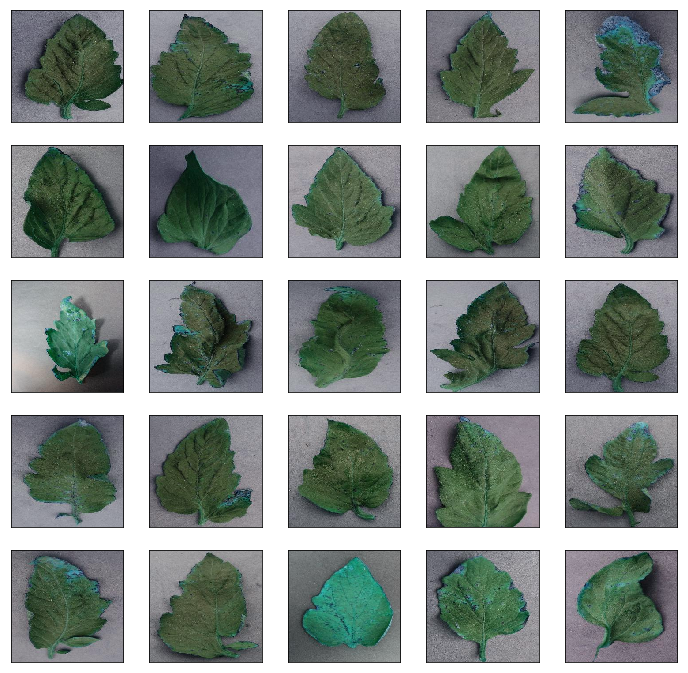
\includegraphics[width=0.46\textwidth]{dataset-plant-village.png}}
\hfill
\subfigure[COCO 2017 background samples]{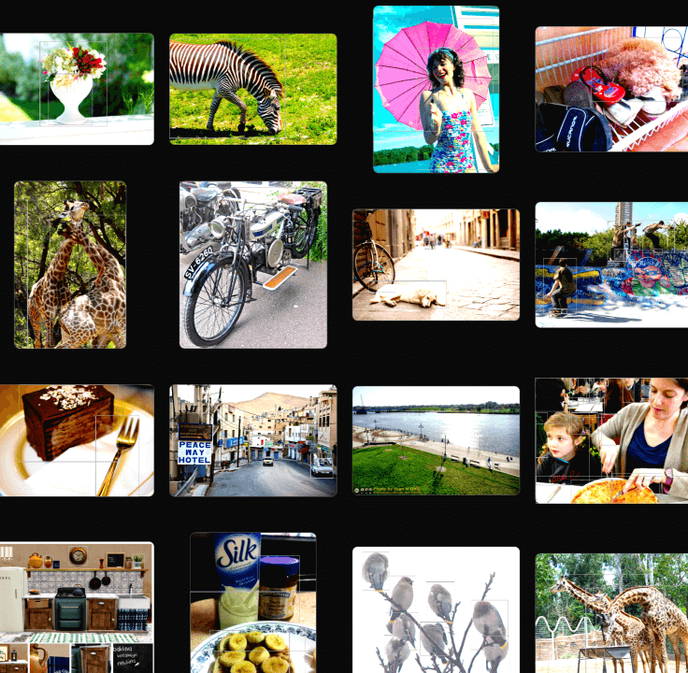
\includegraphics[width=0.46\textwidth]{dataset-coco.png}}
\caption{Dataset sources. Leaf images provide the healthy and diseased classes; non-leaf scenes provide the background class so the model can reject non-leaf input.}
\label{fig:datasets}
\end{figure}
\FloatBarrier

\section{Training pipeline}

Training starts from a \textbf{MobileNet V3-small}~\cite{howard2019mobilenetv3} backbone that has been pretrained on ImageNet, so it already knows general visual features. Only its final classifier head is replaced with a small dropout-plus-linear layer sized to the three target classes, which lets the network adapt to the leaf task while reusing the pretrained features (transfer learning).

Every image is resized to $224\times224$ and normalized with the ImageNet mean and standard deviation, matching the pretrained backbone. During training the data is augmented on the fly with horizontal flips, small ($\pm15^\circ$) rotations, and color jitter, so the model sees slightly varied versions of each leaf and generalizes better. Because the three classes are not equally represented, a weighted sampler is used to draw balanced batches, preventing the model from simply favouring the most common class.

The network is trained for \textbf{15 epochs} with a batch size of \textbf{32}, using the \textbf{Adam} optimizer and a cross-entropy loss. After each epoch the model is checked against the validation set, and only the best-performing checkpoint (lowest validation loss) is kept. That checkpoint is then scored on the held-out test split to report accuracy, per-class metrics, and a confusion matrix.

\IfFileExists{figures/training_pipeline.pdf}{%
  \begin{figure}[H]
  \centering
  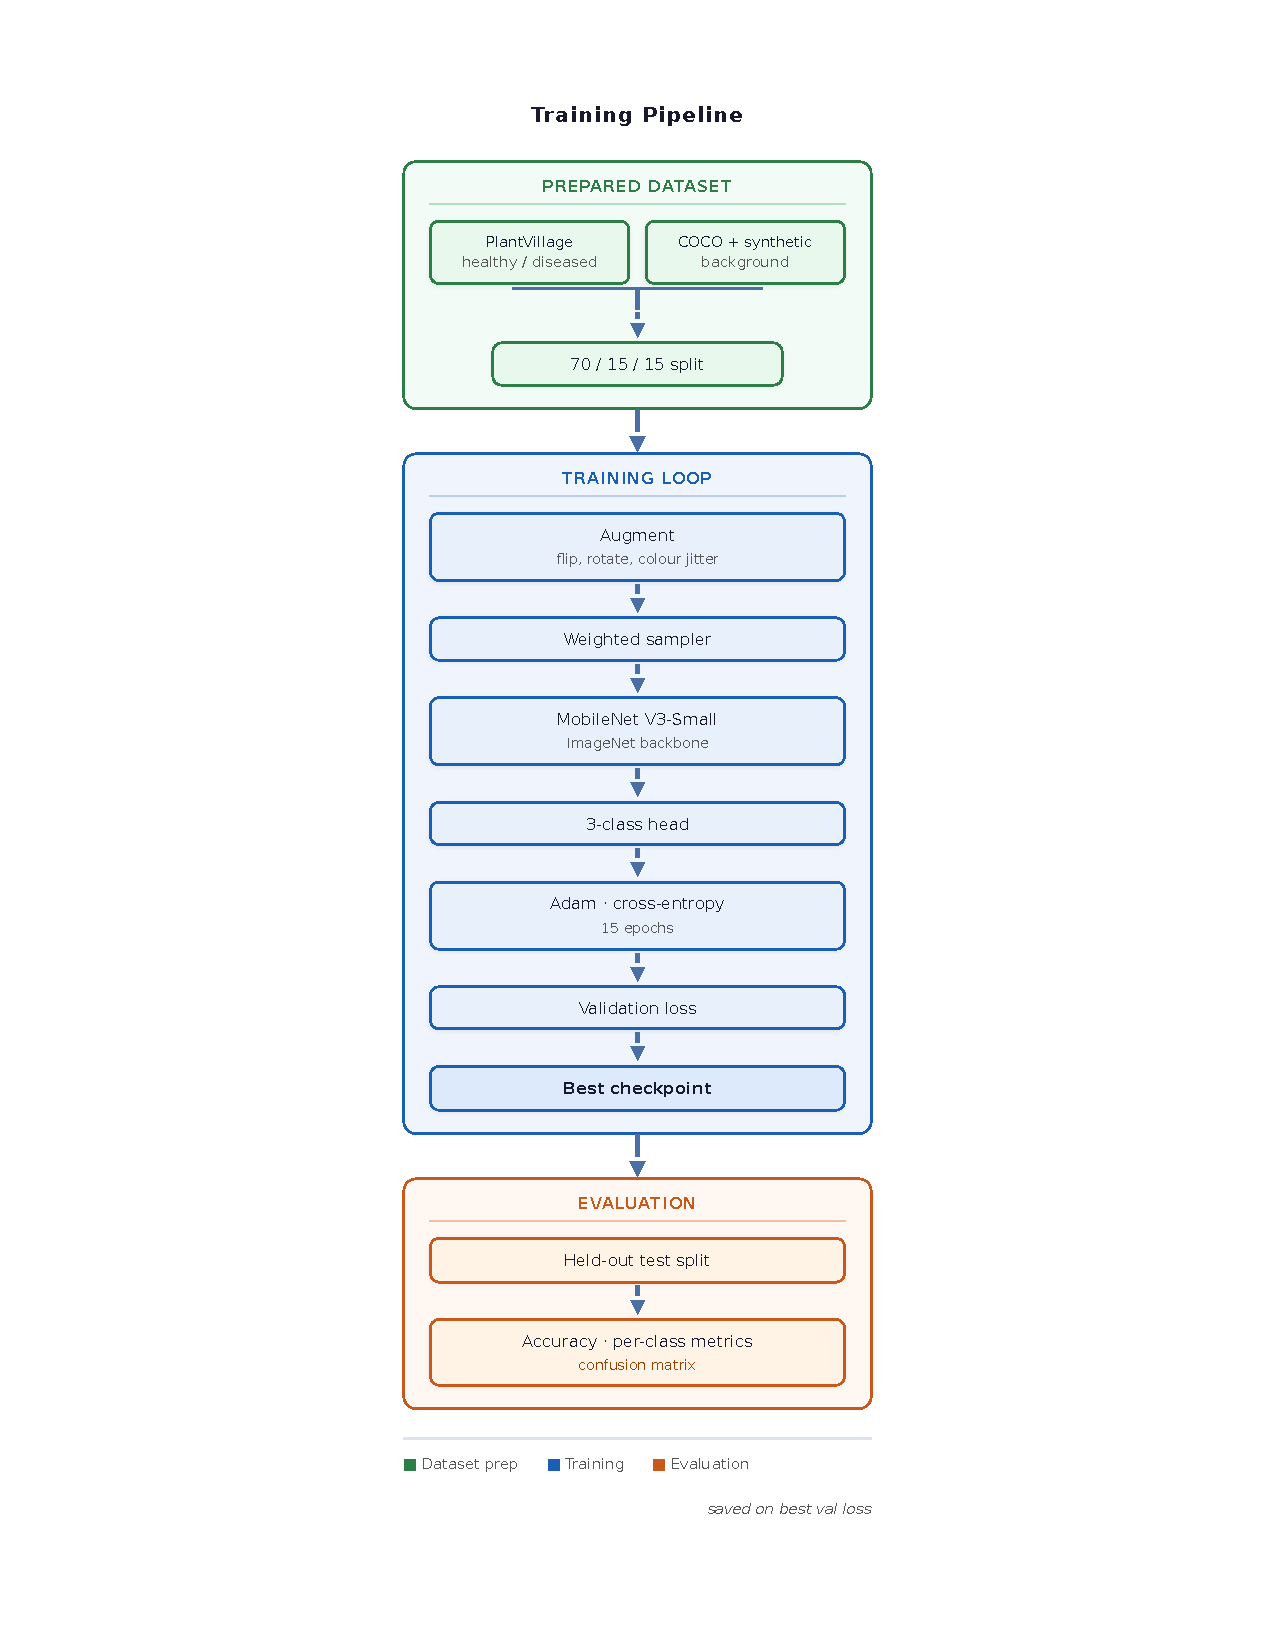
\includegraphics[width=\linewidth,height=0.52\textheight,keepaspectratio]{training_pipeline.pdf}
  \caption{Training pipeline: from the prepared dataset through augmentation and balanced sampling into the pretrained MobileNet V3-small, then validation-based checkpoint selection and held-out evaluation.}
  \label{fig:training-pipeline}
  \end{figure}
}{%
  \begin{quote}
  \textit{Build the figure first: from \path{results/report/}, run \path{./render-mermaid.sh}.}
  \end{quote}
}
\FloatBarrier

\section{ONNX export and quantization}

For deployment, the trained model is converted out of its training framework into \textbf{ONNX}~\cite{onnx}, a portable, framework-independent graph format. The motivation is separation of concerns: training happens in a heavy Python framework, but the device only needs a frozen graph plus a fixed input/output contract (a $224\times224$ image in, three class scores out). ONNX captures exactly that, so the same model can be run by a lightweight native runtime on the Pi without dragging the training stack along. The class names are stored inside the exported model so the runtime always knows what each output means, and a parity check confirms the exported graph produces the same outputs as the original model.

A second, reduced-precision build is also produced through \textbf{INT8 quantization}~\cite{jacob2018quantization}. The idea is that weights and activations, normally stored as 32-bit floats, are mapped to 8-bit integers. This shrinks the model roughly four-fold and lets the CPU use cheaper integer arithmetic, which can speed up inference on suitable hardware. The trade-off is precision: representing values with only 256 levels introduces small rounding errors, so quantized models typically lose a little accuracy. This build is kept as a controlled experiment, evaluated against the full-precision baseline on both accuracy and speed under identical conditions.

\section{On-device runtime (C++)}

The edge stack is implemented in \textbf{C++} with \textbf{ONNX Runtime}~\cite{onnxruntime} so inference stays close to production: no Python interpreter, predictable memory use on 512\,MB RAM, and direct access to ARM NEON for preprocessing.

\textbf{Capture.} The Pi Camera Module 3 feeds frames through the \textbf{libcamera}~\cite{libcamera} stack on Linux. Each frame is converted to an RGB888 buffer suitable for the preprocessor.

\textbf{Preprocessing.} A single fused pass resizes the image to $224\times224$, applies optional channel-order correction, and normalizes with the ImageNet mean and standard deviation into the NCHW layout expected by the exported graph. On aarch64 this path uses \textbf{NEON} vector instructions to keep preprocessing from dominating latency.

\textbf{Inference.} ONNX Runtime loads the frozen MobileNet V3 graph, binds input and output tensors, runs one forward pass per frame, then applies softmax and argmax to obtain the predicted class and per-class probabilities.

\textbf{Serving.} A lightweight HTTP server exposes the web portal at the root URL, an MJPEG preview stream for live video, Server-Sent Events for prediction updates, and a metrics endpoint for CPU load, memory, and temperature. A separate batch-evaluation mode replays labeled folders through the same preprocess-and-infer path to produce the accuracy and throughput numbers reported in the Results chapter.

\IfFileExists{figures/ondevice_runtime.pdf}{%
  \begin{figure}[H]
  \centering
  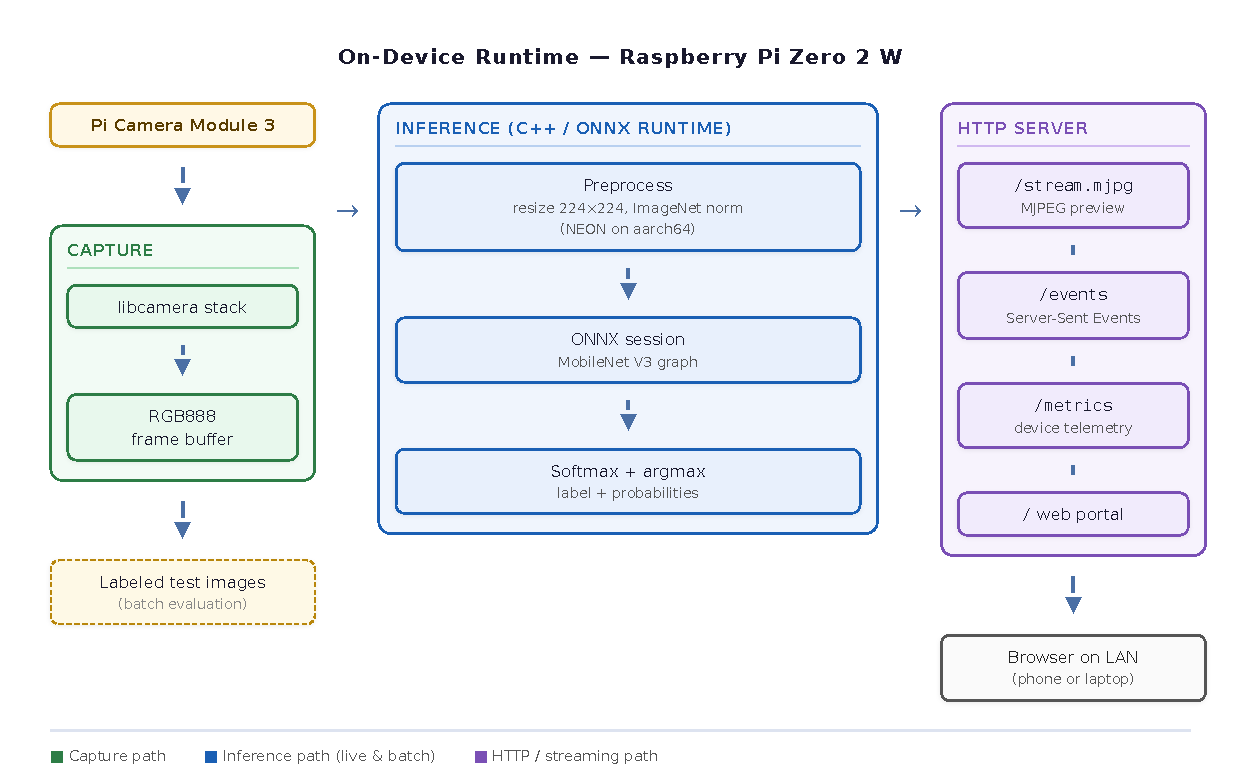
\includegraphics[width=\linewidth,height=0.48\textheight,keepaspectratio]{ondevice_runtime.pdf}
  \caption{On-device runtime: camera capture through preprocessing and ONNX Runtime inference, with HTTP endpoints feeding the browser portal and optional batch evaluation from stored images.}
  \label{fig:ondevice-runtime}
  \end{figure}
}{%
  \begin{quote}
  \textit{Build the figure first: from \path{results/report/}, run \path{./render-mermaid.sh}.}
  \end{quote}
}
\FloatBarrier

\section{Web portal}

The portal is a self-contained web page served from the device on the local network. It shows the live MJPEG camera preview, the predicted label with per-class probability bars, a rolling throughput estimate (FPS), and device health metrics updated about once per second. Operators can point the camera at healthy or diseased leaves and see predictions change in real time; the background class lets the model reject non-leaf scenes instead of guessing.

\begin{figure}[H]
\centering
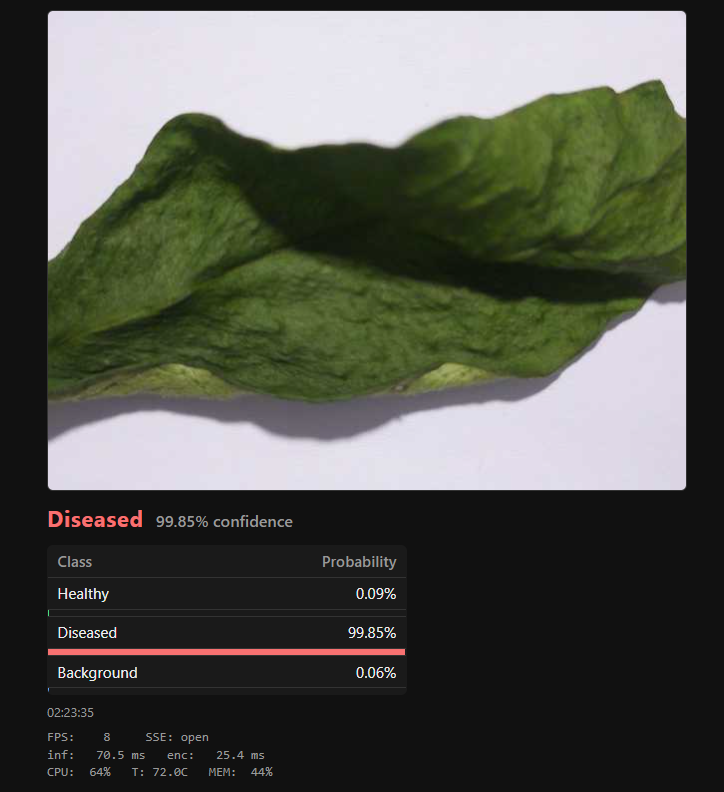
\includegraphics[width=0.65\textwidth]{web-app-diseased.png}
\caption{Web portal: live preview, predicted label with per-class probabilities, FPS, and device metrics.}
\label{fig:web-portal}
\end{figure}
\FloatBarrier

\section{Test bench}

Repeatable field-style testing needs a stable camera pose over leaf samples. A \textbf{3D-printed test bench} (PLA filament) holds the Pi camera at a fixed height and angle above a flat leaf stage, so successive captures share similar framing and lighting.

\begin{figure}[H]
\centering
\subfigure[CAD front]{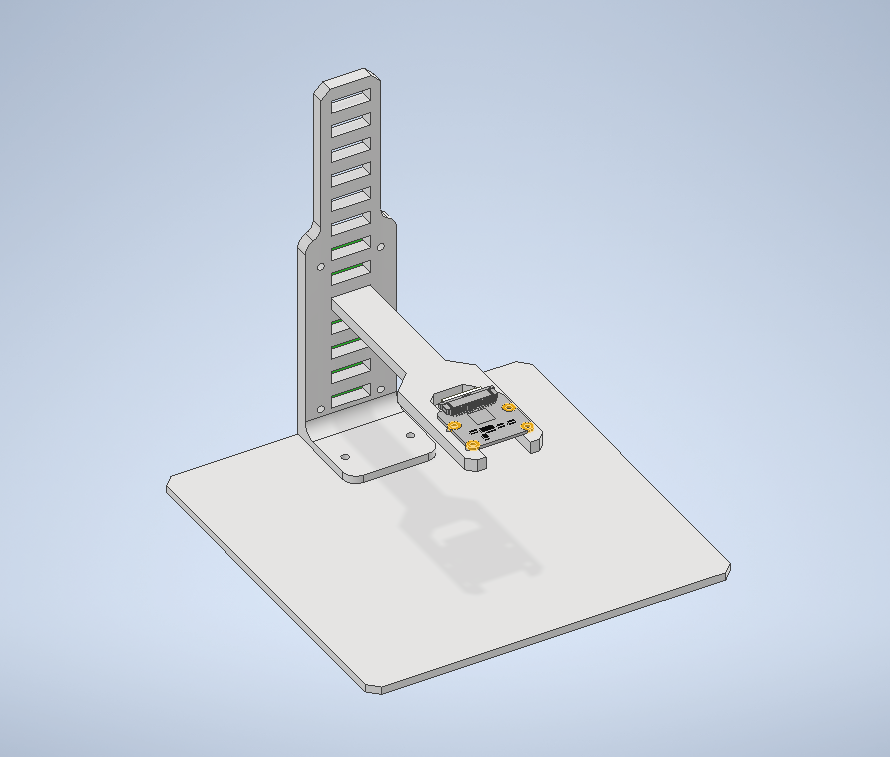
\includegraphics[width=0.42\textwidth]{3d-design-front.png}}
\hfill
\subfigure[CAD back]{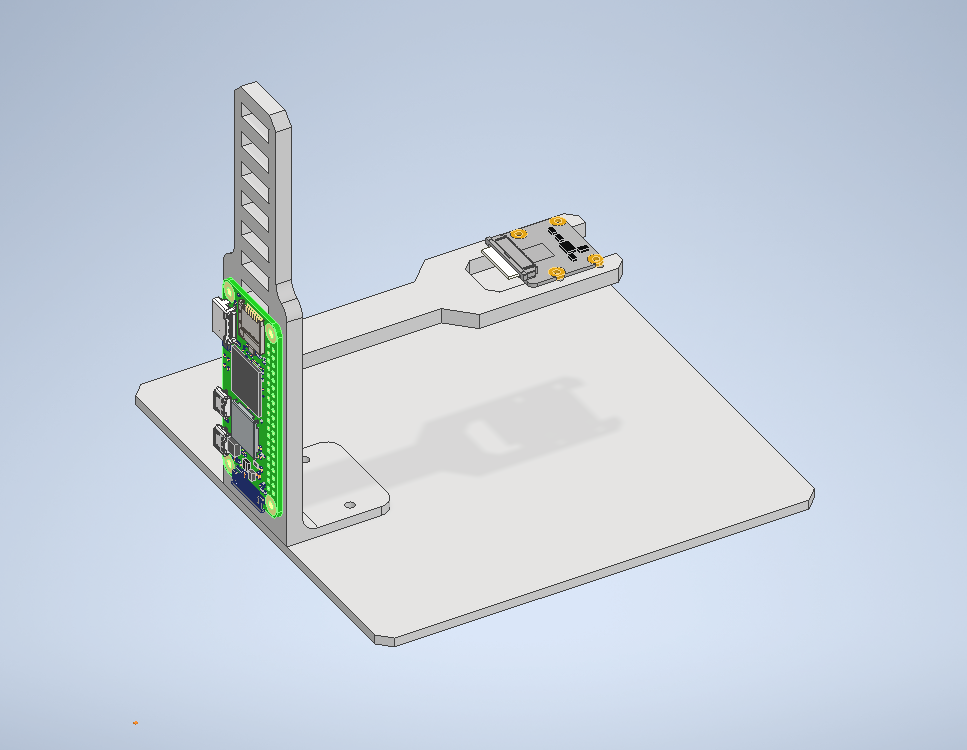
\includegraphics[width=0.42\textwidth]{3d-design-back.png}}
\caption{3D-printed (PLA) test-bench camera stand, CAD model.}
\label{fig:testbench-cad}
\end{figure}

\begin{figure}[H]
\centering
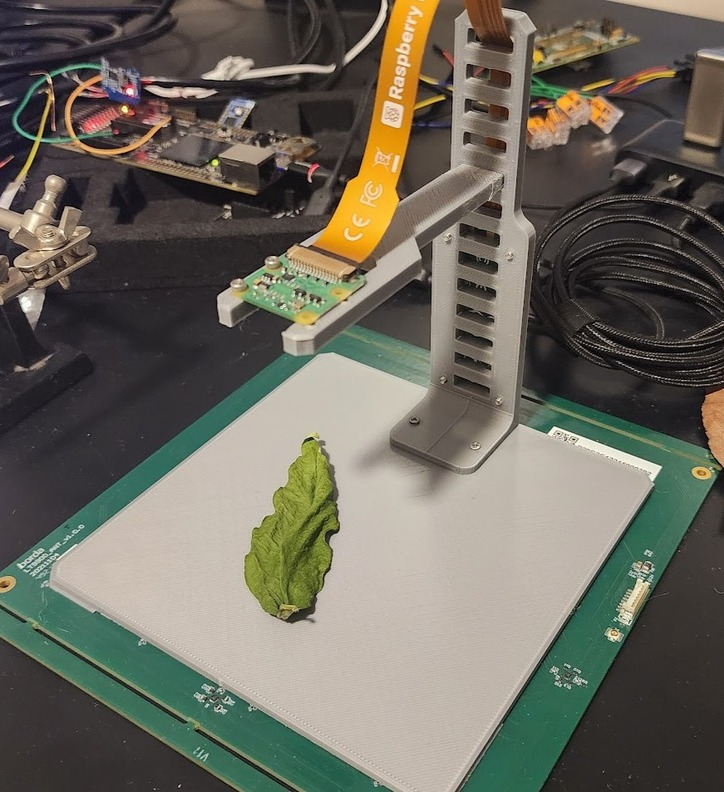
\includegraphics[width=0.6\textwidth]{3d-design-real.jpg}
\caption{Printed test bench in use with the Pi camera and a leaf sample.}
\label{fig:testbench-real}
\end{figure}
\FloatBarrier

\chapter{Results}

This chapter reports \textbf{benchmark-style} runs on the edge device (Raspberry Pi Zero 2 W, ONNX Runtime via native C++) and a \textbf{development workstation} reference (PyTorch on \textbf{CUDA}). On-device runs cover both \textbf{FP32} ONNX and \textbf{INT8/QDQ} ORT builds; sample counts are noted per table (\textbf{8106} images for the 2-class leaf-only split, \textbf{12606} images for the 3-class split that includes the background class).

\section{Pi Zero 2 W -- FP32 (2-class, 8106 images)}

These numbers use \textbf{FP32} ONNX on the leaf-only test split (\textbf{INT8} not used here).

\textbf{Metrics (8106 test images)}

\begin{table}[h!]
\begin{center}
\begin{tabular}{|l|l|}
\hline
\textbf{Metric} & \textbf{Value} \\
\hline
Accuracy & 0.9983 (99.83\%) \\
\hline
Balanced accuracy & 0.9978 (99.78\%) \\
\hline
Precision (diseased) & 0.9988 (99.88\%) \\
\hline
Recall (diseased) & 0.9988 (99.88\%) \\
\hline
F1 (diseased) & 0.9988 (99.88\%) \\
\hline
Specificity (healthy) & 0.9968 (99.69\%) \\
\hline
\end{tabular}
\end{center}
\end{table}

\textbf{Confusion matrix}

\begin{table}[h!]
\begin{center}
\begin{tabular}{|l|r|r|}
\hline
 & \textbf{Pred: healthy} & \textbf{Pred: diseased} \\
\hline
\textbf{Actual: healthy} & 2215 & 7 \\
\hline
\textbf{Actual: diseased} & 7 & 5877 \\
\hline
\end{tabular}
\end{center}
\end{table}

TN: 2215, FP: 7, FN: 7, TP: 5877

\textbf{Speed} (load, preprocess, infer; 8106 images)

\begin{table}[h!]
\begin{center}
\begin{tabular}{|l|l|}
\hline
\textbf{Measure} & \textbf{Value} \\
\hline
Total time & 1009.689 s \\
\hline
Avg / image & 124.561 ms \\
\hline
Throughput & 8.028 img/s \\
\hline
\end{tabular}
\end{center}
\end{table}

\section{Pi Zero 2 W -- FP32 (3-class, 12606 images)}

The full three-class split adds the \textbf{background} class. This run uses \textbf{4 threads}.

\textbf{Overall metrics}

\begin{table}[h!]
\begin{center}
\begin{tabular}{|l|l|}
\hline
\textbf{Metric} & \textbf{Value} \\
\hline
Accuracy & 0.9981 (99.81\%) \\
\hline
Balanced accuracy & 0.9979 (99.79\%) \\
\hline
Macro precision & 0.9971 \\
\hline
Macro recall & 0.9979 \\
\hline
Macro F1 & 0.9975 \\
\hline
\end{tabular}
\end{center}
\end{table}

\textbf{Confusion matrix}

\begin{table}[h!]
\begin{center}
\begin{tabular}{|l|r|r|r|}
\hline
 & \textbf{Pred: healthy} & \textbf{Pred: diseased} & \textbf{Pred: background} \\
\hline
\textbf{Actual: healthy} & 2215 & 5 & 2 \\
\hline
\textbf{Actual: diseased} & 13 & 5871 & 0 \\
\hline
\textbf{Actual: background} & 3 & 1 & 4496 \\
\hline
\end{tabular}
\end{center}
\end{table}

\textbf{Per-class metrics}

\begin{table}[h!]
\begin{center}
\begin{tabular}{|l|r|r|r|r|}
\hline
\textbf{Class} & \textbf{Precision} & \textbf{Recall} & \textbf{F1} & \textbf{Support} \\
\hline
Healthy & 0.9928 & 0.9968 & 0.9948 & 2222 \\
\hline
Diseased & 0.9990 & 0.9978 & 0.9984 & 5884 \\
\hline
Background & 0.9996 & 0.9991 & 0.9993 & 4500 \\
\hline
\end{tabular}
\end{center}
\end{table}

\textbf{Speed} (load, preprocess, infer; 12606 images, 4 threads)

\begin{table}[h!]
\begin{center}
\begin{tabular}{|l|l|}
\hline
\textbf{Measure} & \textbf{Value} \\
\hline
Total time & 801.375 s \\
\hline
Avg / image & 63.571 ms \\
\hline
Throughput & 15.730 img/s \\
\hline
\end{tabular}
\end{center}
\end{table}

\section{Pi Zero 2 W -- INT8/QDQ (3-class, 12606 images)}

The INT8/QDQ ORT build trades a few accuracy points for a smaller footprint. Two runs are reported: a single-thread run and a 4-thread run.

\textbf{Overall metrics}

\begin{table}[h!]
\begin{center}
\begin{tabular}{|l|r|r|}
\hline
\textbf{Metric} & \textbf{INT8 (1 thread)} & \textbf{INT8 (4 threads)} \\
\hline
Accuracy & 0.9721 (97.21\%) & 0.9705 (97.05\%) \\
\hline
Balanced accuracy & 0.9691 (96.91\%) & 0.9667 (96.67\%) \\
\hline
Macro precision & 0.9605 & 0.9588 \\
\hline
Macro recall & 0.9691 & 0.9667 \\
\hline
Macro F1 & 0.9646 & 0.9626 \\
\hline
\end{tabular}
\end{center}
\end{table}

\textbf{Confusion matrix} (INT8, 1 thread)

\begin{table}[h!]
\begin{center}
\begin{tabular}{|l|r|r|r|}
\hline
 & \textbf{Pred: healthy} & \textbf{Pred: diseased} & \textbf{Pred: background} \\
\hline
\textbf{Actual: healthy} & 2106 & 108 & 8 \\
\hline
\textbf{Actual: diseased} & 218 & 5658 & 8 \\
\hline
\textbf{Actual: background} & 3 & 7 & 4490 \\
\hline
\end{tabular}
\end{center}
\end{table}

\textbf{Per-class metrics} (INT8, 1 thread)

\begin{table}[h!]
\begin{center}
\begin{tabular}{|l|r|r|r|r|}
\hline
\textbf{Class} & \textbf{Precision} & \textbf{Recall} & \textbf{F1} & \textbf{Support} \\
\hline
Healthy & 0.9050 & 0.9478 & 0.9259 & 2222 \\
\hline
Diseased & 0.9801 & 0.9616 & 0.9707 & 5884 \\
\hline
Background & 0.9964 & 0.9978 & 0.9971 & 4500 \\
\hline
\end{tabular}
\end{center}
\end{table}

\textbf{Speed} (load, preprocess, infer; 12606 images)

\begin{table}[h!]
\begin{center}
\begin{tabular}{|l|r|r|}
\hline
\textbf{Measure} & \textbf{INT8 (1 thread)} & \textbf{INT8 (4 threads)} \\
\hline
Total time & 2085.312 s & 1282.092 s \\
\hline
Avg / image & 165.422 ms & 101.705 ms \\
\hline
Throughput & 6.045 img/s & 9.832 img/s \\
\hline
\end{tabular}
\end{center}
\end{table}

\section{Dev PC (GPU, reference)}

\textbf{Setup} (example): Ubuntu 24.04 LTS on \textbf{WSL2}; \textbf{CPU}: AMD Ryzen 7 5800H; \textbf{GPU}: NVIDIA GeForce RTX 3050 Laptop (4 GB VRAM).

\textbf{Test metrics}

\begin{table}[h!]
\begin{center}
\begin{tabular}{|l|l|}
\hline
\textbf{Metric} & \textbf{Value} \\
\hline
Accuracy & 0.9980 (99.80\%) \\
\hline
Balanced accuracy & 0.9972 (99.72\%) \\
\hline
Precision (diseased) & 0.9983 (99.83\%) \\
\hline
Recall (diseased) & 0.9990 (99.90\%) \\
\hline
F1 (diseased) & 0.9986 (99.86\%) \\
\hline
Specificity (healthy) & 0.9955 (99.55\%) \\
\hline
MCC & 0.9950 \\
\hline
ROC-AUC & 1.0000 \\
\hline
Parameters & 1,519,906 \\
\hline
\end{tabular}
\end{center}
\end{table}

\textbf{Confusion matrix}

\begin{table}[h!]
\begin{center}
\begin{tabular}{|l|r|r|}
\hline
 & \textbf{Pred: healthy} & \textbf{Pred: diseased} \\
\hline
\textbf{Actual: healthy} & 2212 & 10 \\
\hline
\textbf{Actual: diseased} & 6 & 5878 \\
\hline
\end{tabular}
\end{center}
\end{table}

TN: 2212, FP: 10, FN: 6, TP: 5878

\textbf{Speed} (full eval loop)

\begin{table}[h!]
\begin{center}
\begin{tabular}{|l|l|}
\hline
\textbf{Measure} & \textbf{Value} \\
\hline
Total & 10.7903 s \\
\hline
Avg / image & 1.331 ms \\
\hline
Throughput & 751.23 img/s \\
\hline
\end{tabular}
\end{center}
\end{table}

\section{Summary comparison}

\begin{table}[h!]
\begin{center}
\begin{tabular}{|l|r|r|}
\hline
\textbf{Build (split, threads)} & \textbf{Accuracy} & \textbf{Throughput} \\
\hline
FP32 (2-class, 8106) & 99.83\% & 8.028 img/s \\
\hline
FP32 (3-class, 12606, 4 thr.) & 99.81\% & 15.730 img/s \\
\hline
INT8/QDQ (3-class, 12606, 1 thr.) & 97.21\% & 6.045 img/s \\
\hline
INT8/QDQ (3-class, 12606, 4 thr.) & 97.05\% & 9.832 img/s \\
\hline
\end{tabular}
\end{center}
\end{table}

On the Pi Zero 2 W, \textbf{FP32} keeps accuracy near the reference while \textbf{multi-threading} roughly doubles throughput. The \textbf{INT8/QDQ} build loses about \textbf{2.5--2.7} accuracy points (mostly on the healthy/diseased boundary) and, in this ORT configuration, does not beat multi-threaded FP32 on speed, so FP32 with 4 threads is the strongest on-device operating point measured here.

\chapter{Conclusions and Future Work}

On the \textbf{Pi Zero 2 W}, \textbf{FP32 ONNX} with \textbf{ONNX Runtime} stays accurate on the held-out test set ($\sim$99.8\%) and runs at about \textbf{8 images/s} single-threaded, rising to about \textbf{16 images/s} with four threads on the three-class split. The \textbf{INT8/QDQ} build trades roughly \textbf{2.5--2.7} accuracy points for a smaller artifact but, in this ORT configuration, did not outperform multi-threaded FP32 on throughput; multi-threaded FP32 is therefore the strongest on-device operating point measured here.

\textbf{Why INT8 did not speed up inference.} Quantized INT8 graphs are often faster on CPUs that offer wide integer SIMD or dedicated dot-product instructions (for example x86 VNNI or newer ARM cores with int8 matrix extensions). The Pi Zero 2 W uses a \textbf{quad-core ARM Cortex-A53} (aarch64): it has NEON for \textbf{FP32} float math, but lacks the wider int8 acceleration that many QDQ kernels expect. ONNX Runtime's INT8 path on this core still pays dequantization and requantization overhead around integer ops, so the theoretical savings from 8-bit arithmetic are largely offset. In practice the NEON-friendly \textbf{FP32} kernels remain faster than INT8/QDQ on this hardware.

These results give a solid baseline before further speedups. \textbf{Testing with a real camera in real conditions} still matters, because lab-style test images do not cover everything you see in the field.

\section{Future work}

\begin{itemize}
\item \textbf{Field tests}: systematic runs \textbf{outdoors / in greenhouses} with \textbf{natural lighting} and varied distances, not only dataset-style images, now that the live camera path exists.
\item \textbf{Calibration}: optional score calibration or thresholds for diseased vs healthy when moving from lab to field.
\item \textbf{Speedups}: tune runtime flags and threading for Cortex-A53 to raise images per second.

\bibliographystyle{styles/fbe_tez_v11}
\bibliography{references}



\end{document}
